\scanpage{184}
\[
 \begin{aligned}
 \mathcal A_1&=k\{X_0,X_1,dX_0,dX_1\}/(dX_0+dX_1)_{\mathrm{pd}}\\
 &=k\{T\}\{X_0,\unsure{dX_0}\}\simeq k\{T\}\{X_1,dX_1\}
 \end{aligned}
\]
\figure{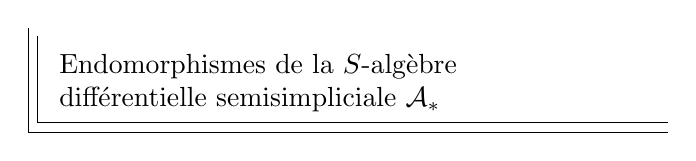
\begin{tikzpicture}
\node[anchor=west,align=left] at (.15,.5) {Endomorphismes de la $S$-algèbre\\différentielle semisimpliciale $\mathcal A_*$};
\draw (0,1.1)--(0,0)--(8,0);\draw (-.12,1.2)--(-.12,-.12)--(8,-.12);
\end{tikzpicture}}
\[
 X_0+X_1=T
\]
\[
 \varphi_1(X_0^{(i)})=\xi_i\qquad
 (1)\quad\boxed{\xi_i\xi_j=c_{ij}\xi_{i+j}}\quad i,j\geq1
\]
\margin{\deleted{$\unsure{(d\xi_1)^2=0}$}}
\[
 \varphi_1(dX_0)=d\xi_1
\]
\inserted{(il est bien de carré nul; il faut encore) et $d\xi_1$ commute aux
$\xi_i$ $(i\geq1)$ \unsure{car} $\mathcal A_1$ \uline{commut.!}}
\diagram{\[
 \begin{array}{ccc}
 \varphi_1(dX_0^{(i)})&=&d\varphi_1(X_0^{(i)})\\
 \text{''}&&\text{''}\\
 \varphi_1(X_0^{(i-1)}dX_0)&&d\xi_i\\
 \text{''}&&\\
 \xi_{i-1}d\xi_1&&
 \end{array}
\]}
\[
 (2)\quad\boxed{d\xi_i=\xi_{i-1}d\xi_1}\quad i\geq2
\]
\margin{On aura
$\varphi_1(d(X_0^{(i)}dX_0))\overset{?}{=}d\varphi_1(X_0^{(i)}dX_0)$
\deleted{$\unsure{\mathcal A_*\simeq k\cdot1}$}
\diagram{\[\begin{array}{cc}
 \text{''}&\text{''}\\
 \varphi_1(0)=0&d(\xi_i d\xi_1)\\
 &\text{''}\\&0
 \end{array}\]}}
\figure{\begin{tikzpicture}\draw[gray] (0,0)--(5.1,0)--(4.65,1.9);\end{tikzpicture}}
\diagram{\begin{tikzcd}[row sep=large]
 \mathcal A_1\arrow[d,bend right=38]\arrow[d,bend left=38,"\beta"]\\
 \mathcal A_0=k\{T\}
\end{tikzcd}}
\[
 \left\{\begin{aligned}
 \alpha(X_0^{(i)})&=0&&\forall i\geq1\\
 \alpha(dX_0)&=0
 \end{aligned}\right.
 \qquad
 \begin{aligned}
 \beta(X_0^{(i)})&=T^{(i)}&&\forall i\geq1\\
 \beta(dX_0)&=0
 \end{aligned}
\]
\[
 \left\{\begin{aligned}\alpha\circ\varphi_1&=\alpha\\\beta\circ\varphi_1&=\beta\end{aligned}\right.
\]
\[
 \begin{array}{ll}
 \alpha\circ\varphi_1(\unsure{X^{(i)}|X_0^{(i)}})=\alpha(\xi_i)&
 \text{\textcircled{3a}}\quad\boxed{\alpha(\xi_i)=0}\\
 \alpha(\unsure{X^{(i)}|X_0^{(i)}})=0&\\
 \beta\circ\varphi_1(X^{(i)})=\beta(\xi_i)&
 \text{\textcircled{3b}}\quad\boxed{\beta(\xi_i)=T^{(i)}}\\
 \beta(X^{(i)})=T^{(i)}&
 \end{array}
\]
\[
 \xi_i=\overbrace{\sum_{j\geq0}a_{ij}\deleted{\unsure{T}}X_0^{(j)}}^{A_i}
 +\overbrace{\left(\sum_{j\geq0}b_{ij}X_0^{(j)}\right)}^{B_i}dX_0
 \qquad \unsure{a_{ij}|a_j},b_{ij}\in k\{T\}
\]
(3a) s'écrit
\figure{\begin{tikzpicture}\node[draw,ellipse] {$a_{i,0}=0\quad\forall i\geq1$};\end{tikzpicture}}
\textcircled{3'a}\quad i.e.
\figure{\begin{tikzpicture}\node[draw,ellipse] {$A_i=\sum_{j\geq1}a_{ij}X_0^{(j)}$};\draw[->] (-2,.2)..controls(-2.3,.4)and(-2.45,.55)..(-2.3,.7);\end{tikzpicture}}
$\forall i\geq1$

(3b) s'écrit
\deleted{$\unsure{\sum_{j\geq1}a_{ij}X_0^{(j)}}\equiv$}
\textcircled{3'b}
\figure{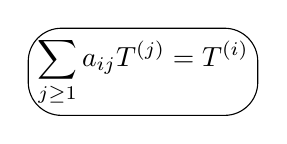
\begin{tikzpicture}\node[draw,rounded corners=12pt] {$\displaystyle\sum_{j\geq1}a_{ij}T^{(j)}=T^{(i)}$};\end{tikzpicture}}
$\forall i\geq1$
\[
 d\xi_i=\left(\sum_{j\geq1}a_{ij}X_0^{(j-1)}\right)dX_0
 =\deleted{\unsure{d\xi_i=dA_i}}
\]
\[
 d\xi_1=\left(\sum_{j\geq1}a_{1j}X_0^{(j-1)}\right)dX_0
\]
\[
 \xi_{i-1}=\sum_{j\geq1}a_{i-1,j}X_0^{(j)}
 +\left(\sum_{j\geq0}b_{i-1,j}X_0^{(j)}\right)dX_0
\]
\[
 \xi_{i-1}d\xi_1=
 \left(\sum_{k\geq1}a_{1k}X_0^{(k-1)}\right)
 \left(\sum_{\unsure{\ell}\geq1}a_{i-1,\unsure{\ell}}X_0^{(\unsure{\ell})}\right)dX_0
\]
\margin{183}
